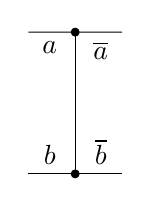
\begin{tikzpicture}[auto, scale=0.3]
	
	\node (bA) [scale=0.03] at (13, 6) {};
    \node (b1) [circle, draw, fill, scale=0.3] at (15, 6) {};
    \node (b2) [scale=0.03] at (17, 6) {};
    
    \node (bB) [scale=0.03] at (13, 0) {};
    \node (b7) [circle, draw, fill, scale=0.3] at (15, 0) {};
    \node (b8) [scale=0.03] at (17, 0) {};
    
    \path[-]
    (bB) edge node[above] {$b$} (b7)
    (bA) edge node[below] {$a$} (b1)
    (b2) edge node[below] {$\overline{a}$} (b1)
    (b7) edge node[above] {$\overline{b}$} (b8)
    (b1) edge (b7);
    
\end{tikzpicture}
